% GitHub cvitanov/reducesymm/QFT/exponThe.tex
% to compile:  cd cvitanov/reducesymm/QFT; pdflatex blog; biber blog

% Predrag  created              Dec 23 2018

\section{Non-Abelian exponentiation theorem}
\label{s:FiMaFu18}
\newcommand{\vev}[1]{{\left< {#1} \right>}}

{\bf [2018-12-22 Predrag]}

% Bartomeu Fiol <bfiol@ub.edu>,  jmartinez@icc.ub.edu, ariosfukelman@icc.ub.edu
Fiol, Martínez-Montoya and Fukelman\rf{FiMaFu18} {\em Wilson loops in
terms of color invariants} addresses the question of whether one can
compute directly the logarithm of $\vev{W}_R$, the vacuum expectation
value (vev) of a Wilson loop.

The reason I'm intrigued by this paper is that their `$n$-gluon chord
diagrams' are also the $n$-photon, no-fermion loop `quenched-'
% , or `q-type'
diagrams
% (`quenched', as this corresponds to the $N_f$-independent part
% of the vertex amplitude in QED with $N_f$ flavors)
of the quenched QED in the worldline formalism. So far, in the worldline
formalism we are looking at what corresponds to $\vev{W}_R$ chord
diagrams, but we need only the $\ln \vev{W}_R$ connected diagrams, and really
its Legendre transform, the 1pI diagrams. I would generate $\ln
\vev{W}_R$ using Dyson-Scwinger equations for connected correlation
functions, see the relations between the full generating function $Z[J]$,
the connected generating function $W[J]$, and the 1pI generating function
$\Gamma[\phi]$ in \refref{FieldThe}.

They show that the \emph{non-Abelian exponentiation
theorem}\rf{Gatheral83,FreTay84} implies that certain color invariants
present in $\vev{W}_R$ are absent in $\ln \vev{W}_R$. To me this looks
like the connection between the full and connected partition functions,
except that here quark lines are not providing connections, only the
crossed gluon lines are. The relation is the simplest one possible:
Wilson loop is always connected, but the color weight of any subdiagram
that looks like a self-energy insertion factorizes, so we are looking at
rewriting the vev in terms of graphs with no self-energy insertions, as
in the `complete propagator' $W''$ of eq.~(2.32) of \refref{FieldThe}.

Fiol \etal\rf{FiMaFu18} start by evaluating the integrals over the full
Lie group G of the ${\cal N}=4$ super Yang Mills matrix model:
\beq
\vev{W}_R = \frac{1}{d_R}\vev{\tr\, e^{2\pi M}}=
 \frac{1}{d_R} \frac{
    \int_{\mathfrak{g}}dM\,\tr\,e^{2\pi M}\,e^{-\frac{2\pi^2}{g}{\scriptsize \tr}M^2}
                    }{
    \int_{\mathfrak{g}}dM\,e^{-\frac{2\pi^2}{g}{\scriptsize \tr}M^2}
                     }
\,,
\ee{winmm}
where $g=g^2_\text{YM}/4$ is a Yang-Mills ``fine structure'' constant
(up to $\pi$'s factors  here and there).
Denoting by $m^a$ the coefficients of the matrix $M$ in the Lie algebra,
the two-point function in this Gaussian matrix model is
\beq
\vev{m^a m^b}= \frac{g}{2\pi^2}\,\delta^{ab} \hspace{1cm} a,b=1,\dots, N
\,.
\ee{atwopoint}
To compute the vev of the normalized Wilson loop, expand $\exp(2\pi M)$
in \refeq{winmm}, use the two-point function \refeq{atwopoint}, and apply
Wick's theorem. The vev of $W_R$ is given by symmetrized traces with
pairwise contracted indices,
\bea
\vev{W}_R
&=& \frac{1}{d_R}\sum_{k=0}^\infty
    \frac{(2\pi)^{2k}}{(2k)!} \vev{m^{a_1}\dots m^{a_{2k}}}\,
                          \tr T^{a_1}_R \dots T^{a_{2k}}_R
        \continue
&=& \frac{1}{d_R}\sum_{k=0}^\infty
    \frac{1}{k!} d_R^{a_1a_1\dots a_k a_k} g^k
\,,
\label{exactvev}
\eea
where $d_R^{a_1\dots a_k}$ are the fully symmetrized traces
\beq
d_R^{a_1\dots a_n}
  =\frac{1}{n!} \sum_{\sigma \in {\cal S}_n}
                \tr\,T_R^{a_{\sigma(1)}}\dots T_R^{a_{\sigma (n)}}
\,,
\ee{symtraces}
and $T^a_R$ are the generators of the Lie algebra of the group G in
the representation R.
$d_R$ with no superscript is the trace of the identity matrix,
$d_R=\tr\,{\bf 1}= \text{dim }R$.

`Casimirs' \refeq{symtraces} are studied in Chaper~7 of \refref{PCgr};
% and some in \refref{NPB81};
perhaps re-expressing color invariants in terms of orthogonal Dynkin
indices might yield some extra insights.
For \Un{1} of the (quenched) QED, the Lie algebra is one\dmn, all
$T_R^{a_j}=1$, and all $d_R^{a_1\dots a_n}=1$.

Expression \refeq{exactvev} yields exact relations among vevs in different
representations. For instance, if $\transp{R}$ is the transpose representation
of $R$ corresponding to a transpose Young diagram, then, following
\refrefs{NegDimE7,CK82,PCgr},
\[
\vev{W}_{\transp{R}}(\lambda,n)=\vev{W}_R(\lambda,-n)
\,.
\]
This relates the vevs in the symmetric and the antisymmetric
representations of \SUn{n}, and makes irreps self-dual under Young
diagram transposition functions of $n^2$.
For \SUn{n} fully (anti)symmetric irrep there is an intriguing
factorization, their eq.~(2.11).

The evaluation of the fully symmetrized traces \refeq{symtraces} with
pairwise contracted indices $d_R^{a_1 a_1\dots a_k a_k}$ (for example
$d_R^{aabb}$) yields combinations of lower order color invariants (for
example $d_R^{abcd}d_A^{abcd}$).
At low orders they evaluate them by hand, using the methods of van
Ritbergen, Schellekens and Vermaseren {\em Group theory factors for
{Feynman} diagrams}\rf{RiScVe99}, \arXiv{hep-ph/9802376},
\begin{align*}
d_R^{aa} & = \tr\,T_R^a T_R^a= c_R d_R \\
d_R^{aabb} & =  \frac{1}{3}\tr\,
\left(2T_R^aT_R^aT_R^bT_R^b+T_R^aT_R^bT_R^aT_R^b\right)
=(c_R^2-\frac{1}{6}c_A c_R)d_R
\end{align*}
Higher orders, up to order $g^{7}$, they evaluate using
FormTracer\rf{CyMiSt16}.
Fiol \etal\rf{FiMaFu18} conventions for color invariants are largely
those of van Ritbergen, Schellekens and Vermaseren.
Some of the invariants are given by Okubo and Patera {\em General indices
of simple {Lie} algebras and symmetrized product
representations}\rf{OkuPat83}.
These expressions are not pretty, but
fortunately the perturbative expansion of $\ln \vev{W}_R$ is considerably
simpler.

Explicit computation of $\ln \vev{W}_R$ up to order $g^{7}$ demonstrates
that $\ln \vev{W}_R$ is simpler than that of $\vev{W}_R$. Many color
invariants present in the expansion of $\vev{W}_R$ are absent in the
expansion of $\ln \vev{W}_R$. For instance, there are no color invariants
involving the quadratic casimir $c_R^k$ with $k\geq 2$: the only color
invariants that appear in the perturbative expansion of $\ln \vev{W}_R$
at a given order are those that cannot be written as products of color
invariants that appear at lower orders of the perturbative expansion,
thus providing an illustration of the non-Abelian exponentiation
theorem\rf{Gatheral83,FreTay84}.

The non-Abelian exponentiation theorem offers some support to the
conjecture of
Fiol, Gerchkovitz and Komargodski\rf{FiGeKo16}
{\em Exact bremsstrahlung function in {N}=2 superconformal field theories}.
A closed formula for the bremsstrahlung function is given in terms of a
derivative with the respect to the coupling,
\beq
B_R(\lambda,n)
=\frac{1}{2\pi^2}\lambda \frac{\partial \ln \vev{W}_R}{\partial \lambda}
= \cdots
\ee{closedb}
due to $\ln \vev{W}_R$, only a subset of the most general color
invariants appears in the expansion of the bremsstrahlung function $B$.
This formula is worth remembering when thinking of the self-energy vs.
vertex diagram computation of the anomalous magnetic moment.

\medskip

Very interesting is their diagrammatic interpretation of the perturbative
expansion of $\ln \vev{W}_R$. According
\refrefs{ErSeZa00,DruGro01,Pestun12}, \arXiv{hep-th/0003055},
\arXiv{hep-th/0010274}, \arXiv{0712.2824}, the only Feynman diagrams that
contribute to $\vev{W}_R$ in the Feynman gauge involve gluon propagators
starting and ending on the Wilson line. Such diagrams are called
\emph{chord diagrams}\rf{Touchard52} (note that all gluons are drawn on
the same side of the quark line). At order $2n$ there are $(2n-1)!!$ of
them. On the other hand, by virtue of the non-Abelian exponentiation
theorem\rf{Gatheral83,FreTay84}, to compute $\ln \vev{W}_R$ one only
needs to take into account a subset of them, the so-called
\emph{connected chord diagrams}: diagrams where all gluon lines overlap
with some other gluon line, see \reffig{f:FiMaFu181f}.

\begin{figure}
\centering
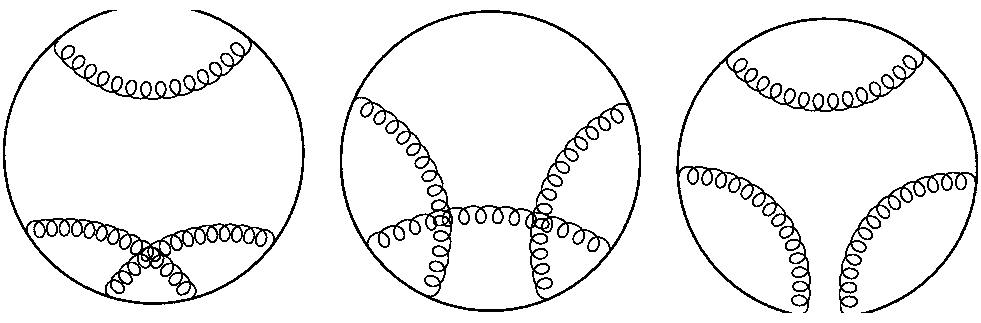
\includegraphics[width=.8\textwidth]{FiMaFu181f}
\caption{
Examples of chord diagrams (note that all gluons are drawn on the same
side of the quark line). The second one is a connected chord diagram.
They contribute to $\ln \vev{W}_R$.
The last diagram is a fully disconnected chord diagram. For $k$ gluons,
there are ${\cal C}_k= {(2k)!}/{(k+1)! k!}$ of them.
(From Fiol \etal\rf{FiMaFu18})
        }
\label{f:FiMaFu181f}
\end{figure}

The number of connected chord diagrams with $n$ chords satisfies the
recursion relation\rf{Stein78,NijWil79}
\beq
a_1=1 \hspace{1cm} a_n =(n-1)\sum_{k=1}^{n-1} a_k a_{n-k}
\,,
\ee{connectedchord}
so up to seven loops the numbers are
\[
a_n=1,1,4,27,248,2830,38232,\dots
\]
Asymptotically the ratio of the number of connected chord diagrams to the
total number of chord diagrams with $n$ gluons (or photons)
is $e$ times less than the total number of Feynman diagrams\rf{SteEve78},
\[
\lim_{n\to \infty} \frac{a_n}{(2n-1)!!}=\frac{1}{e}
\,.
\]
This might be (never thought of it this way?) simply the full to the
connected partition functions relation
$Z[J]=\exp W[J]$.

To compute $\ln \vev{W}_R$ by evaluating the connected gluon diagrams
according to the non-Abelian exponentiation
theorem\rf{Gatheral83,FreTay84}, the color weight of each diagram is a
modified color weight $\bar c_i$. To compute $\bar c_i$ of a given
connected gluon diagram, one has subtract the color weights of all
possible gluon insertions of the diagram, as illustrated in
\reffig{f:FiMaFu18modCFac}.

\begin{figure}
  \centering
  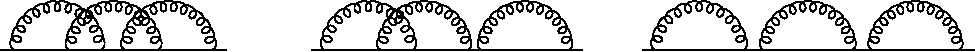
\includegraphics[width=1\textwidth]{FiMaFu18modCFac}
  \put(-263,2){\Large$-$\Huge$($}
  \put(-245,2){\LARGE$2$}
  \put(-132,2){\Large$+$}
  \put(0,2){\Huge$)$}
  \put(-290,-30){\large$\bar c= c_R \left( c_R - \frac{1}{2} c_A \right)^2 -  \left( 2c_R(-\frac{1}{2}c_R c_A)+c_R^3 \right)= \frac{1}{4} c_R c_A^3$}
  \caption{
The modified color weight of this connected 3-gluon diagram is obtained
by subtracting from its color weight all other gluon insertions.
(From Fiol \etal\rf{FiMaFu18})
    }
\label{f:FiMaFu18modCFac}
\end{figure}

Two chord diagrams have the same reduced color weight if their
intersection graphs are isomorphic. An \emph{intersection graph} is
defined as follows\rf{Bouchet94} (note that all gluons are drawn on the
same side of the quark line): for each chord place a point on the plane;
if two chords cross, draw an edge between the two points, see
\reffig{f:FiMaFu186c} (note that all gluons are drawn on the same side of
the quark line). Since only connected chord diagrams contribute to $\ln
\vev{W}_R$, one needs to consider only the connected intersection graphs.
If $n$ is the number of gluon propagators, Fiol \etal\ have (compare to
\refeq{symtraces})
\[
\ln \vev{W}_R= \sum_{n=1}^\infty \frac{1}{2n!}
\left(2 g^2\right)^n \sum_{conn} \bar c_i
\]
where the sum runs over connected chord diagrams with $n$ gluon
propagators.

The numbers of non-isomorphic connected intersection graphs for chord
diagrams are\rf{ArBeCoSo00}
\[
1,1,2,6,21,110,789,8336,117283,\dots
\]
At order $g^4$, there are $7!!=105$ 4-gluon chord diagrams, 27 connected
chord diagrams, and 6 connected intersection graphs. In detail,
the 27 connected chord diagrams are grouped according to
six intersection graphs as $27=8+4+8+2+4+1$.
The reduced color weights that they list up to four loops, with
intersection graph up to four dots, are surprisingly simple.

\begin{figure}
\centering
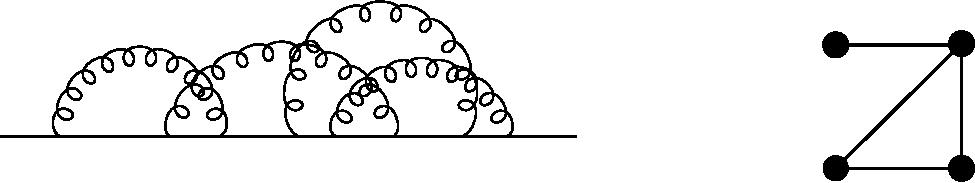
\includegraphics[width=.8\textwidth]{FiMaFu186c}
\caption{
The intersection graph of a 4-gluon Feynman diagram. For each gluon, draw
a dot on the plane; each time two gluon lines intersect, draw a link
between the corresponding dots.
(From Fiol \etal\rf{FiMaFu18})
    }
\label{f:FiMaFu186c}
\end{figure}


Starting at seventh order, color invariants are not all independent; the
first identity they satisfy is\rf{RiScVe99}
\beq
d_A^{abcdef}d_A^{abcdef}-\frac{5}{8}d_A^{abcd}d_A^{cdef}d_A^{efab}
+\frac{7}{240}c_A^2 d_A^{abcd}d_A^{abcd}+\frac{1}{864}c_A^6 d_A
=0
\,.
\ee{adjointrelation}
They indulge in a bit of intriguing but so far inconclusive numerology,
much of it requiring extra thinking starting with the seventh order.




%%%%%%%%%%%%%%%%%%%%%%%%%%%%%%%%%%%%%%%%%%%%%%%%%%%%%%%%%%%%%%%%%%%%%%%%%%%
\Remarks

\remark{Non-Abelian exponentiation theorem.}{\label{rem:exponTheLit}
The literature on the non-Abelian exponentiation\rf{Gatheral83,FreTay84} is huge.

I like White\rf{White16} {\em An introduction to webs} which is
pedagogical, and path integral (generating function) based.
Instead of the field theory of a single soft photon, one considers a
theory with $N$ non-interacting identical copies, or \emph{replicas}, of
the soft gauge field. The replica trick is an explicit procedure
for determining  $\log Z$; in other words, for determining which
diagrams exponentiate in the non-replicated theory.

While eikonal approximation seems not to include
self-energy type insertions, we could think of replicas building up our
$(k,m,m')$ sets.

In his 2019 lecture
\HREF{https://www.ipht.fr/Meetings/Itzykson2014/talks/Gardi-Itzykson19.pdf}
{Gardi} explains it on p.~19:
``Diagrams contributing to the exponent (webs) have a non-Abelian color
factor and no subdivergences.''
Webs
have only  two-eikonal line irreducible subdiagrams.
``Theorem\rf{GaSmWh13}: all color structures in the exponent correspond
to connected graphs.'' But the lectures are about the multi-Wilson lines -
we need only two, or a ``cusp,'' so ignore these lectures.

``Key observation:
Exponentiation of connected subdiagrams looks like
exponentiation of connected diagrams in QFT.
They are related, after rewriting of the problem.''
They talk about ``first-quantised path integral, where $x(t)$ is the
trajectory of the particle,'' \ie, wordline formalism.

Extension to fermion emitting particles is straightforward.
 Get extra terms in classical action, which have spinor
structure (magnetic moment vertices).

The eikonal approximation corresponds to neglecting recoil \ie\
$x(t)$ is the straight-line classical trajectory.

The physics of this approximation is that soft gluons, as discussed
above, have an infinite Compton wavelength. Thus, they are not able to
resolve the internal details of the hard interaction, which consequently
appears pointlike.
Due to its large Compton wavelength, a soft photon cannot resolve the
magnetic moment of the emitting particle, hence is insensitive to the
spin. The magnetic moment vertex
contributes first to the NE (next-to eikonal
exponentiation).

``Virtual amplitudes in eikonal approximation are exponentials of simpler
quantities, which only receive contributions from diagrams whose color
weights are those of `single connected webs' (maximally
non-abelian)\rf{Gatheral83,FreTay84}.''
``Purely virtual amplitudes in eikonal (\ie, soft-gluon) approximation
can be written as exponentials of simpler quantities, which receive
contributions only from Feynman diagrams whose color weights are
`color-connected' (or `maximally non-abelian'). Only color structures
consisting of a single connected web contribute to the exponent.''
``Interesting new webs involving higher casimirs appear first at four
loops.''
Color conservation reduces the six possible color weights to three of
which $d_R^{aabb}$ is not reducible to already known weights (\ie,
quadratic casimir). Applied to the two-jet case (form factors), massless
partons (of no interest to use here), this implies Casimir scaling of the
cusp anomalous dimension. For the purely massive case, all structures
allowed by non-Abelian exponentiation at a given order will be present.

Laenen, Stavenga and White\rf{LaStWh09}
{\em Path integral approach to eikonal and next-to-eikonal exponentiation},
is summarized in White's
\HREF{https://indico.desy.de/indico/event/1766/session/7/contribution/36/material/slides/0.pdf}
{lecture} {\em QCD: The Modern View of the Strong Interactions}.

There is so much literature just to check, I give up her for now.
Just do it, blog here if you learn anything of interest:

\HREF{https://doi.org/10.1016/0370-2693(92)90405-S} {10.1016/0370-2693(92)90405-S}

\HREF{https://doi.org/10.1016/j.nuclphysb.2007.11.002} {10.1016/j.nuclphysb.2007.11.002}

\HREF{https://doi.org/10.1016/j.nuclphysb.2007.11.007} {10.1016/j.nuclphysb.2007.11.007}

\arXiv{0810.2183}

\HREF{https://doi.org/10.1088/1126-6708/2009/03/054} {10.1088/1126-6708/2009/03/054}

\HREF{https://doi.org/10.1088/1126-6708/2009/11/062} {10.1088/1126-6708/2009/11/062}

\HREF{https://doi.org/10.1134/s0040577917030035} {10.1134/s0040577917030035}

\HREF{https://doi.org/10.1007/JHEP03(2011)079} {10.1007/jhep03(2011)079}

\HREF{https://doi.org/10.1007/jhep04(2014)044} {10.1007/jhep04(2014)044}

\HREF{https://doi.org/10.1007/jhep06(2015)120} {10.1007/jhep06(2015)120}

\HREF{https://doi.org/10.1007/jhep10(2016)130} {10.1007/jhep10(2016)130}

\HREF{https://doi.org/10.1007/JHEP11(2010)155} {10.1007/jhep11(2010)155}

\HREF{https://doi.org/10.1007/jhep12(2016)121} {10.1007/jhep12(2016)121}

\HREF{https://doi.org/10.1007/s00601-017-1327-x} {10.1007/s00601-017-1327-x}

\HREF{https://www.groundai.com/project/exponentiation-for-products-of-wilson-lines-within-the-generating-function-approach/} {groundai.com/project/exponentiation-for-products-of-wilson-lines-within-the-generating-function-approach/}

\HREF{https://doi.org/10.1103/PhysRevD.90.066007} {10.1103/PhysRevD.90.066007}

Possibly Les Houches lectures by
\HREF{http://personalpages.to.infn.it/~magnea/} {Lorenzo Magnea}
{\em Eikonal Correlators and form factors in perturbation
theory}
(search for comment {\bf 2018-06-10 Predrag}),
and
\HREF{https://www.nikhef.nl/pub/theory/people.html} {Franz Herzog}
{\em Geometric IR subtraction in real radiation}
were about this.


    } %end Non-Abelian exponentiation theorem

\RemarksEnd
